\documentclass{IEEEtran}
\usepackage{graphicx}
\usepackage{fancyhdr}
\usepackage{verbatim}

\graphicspath{ {images/} }
\pagestyle{fancy}
\fancyhf{}
\rhead{Primer Proyecto Programado}
\rfoot{P\'agina \thepage}

\begin{document}
\begin{titlepage}
  \centering
  {\scshape\LARGE Instituto Tecnol\'ogico de Costa Rica \par}
  \vspace{1cm}
  {\scshape\Large Primer proyecto programado\par}
  \vspace{1.5cm}
  {\Large\itshape Ariel Herrera\par}
  {\Large\itshape Sa\'ul Zamora\par}
  \vfill
  profesor\par
  M. Sc. Sa\'ul Calder\'on Ram\'irez \textsc{}

  \vfill

% Bottom of the page
  {\large \today\par}
\end{titlepage}

\section{Introducci\'on}

El an\'alisis de contenido de video o en ingl\'es \emph{Video Content Analysis, Video Content Analytics o VCA} es la habilidad de analizar autim\'aticamente un video para determinar eventos temporales y/o espaciales.

Esta capacidad t\'ecnica es usada en un amplio rango de dominios, los cuales incluyen entretenimiento, cuidados de la salud, ventas, automotores, transporte, automatizaci\'on de hogares, detecci\'on de fuego y humo, seguridad, entre otros. Los algoritmos pueden ser implementados por software en m\'aquinas de prop\'osito general o en hardware especializado en procesar unidades de video.

Muchas funcionalidades distintas pueden ser implementadas en VCA. Detecci\'on de movimiento en video es una de las formas m\'as simples en las que el movimiento es detectado respecto a una escena de fondo inm\'ovil.

VCA depende de video de buena calidad como entrada, as\'i que usualmente es combinado con tecnolog\'ias de mejoramiento de video como super resoluci\'on, estabilizaci\'on de imagen, entre otros.

\section{An\'alisis del problema}

Actualmente la Universidad de Costa Rica desarrolla un sistema de an\'alisis de video con el fin de analizar autom\'aticamente videos de futbol. Las etapas de \'este van desde la identificaci\'on de escenas con informaci\'on \'util en el video, segmentaci\'on y rastreo de jugadores, hasta el an\'alisis autom\'atico de los recorridos y comportamiento de los jugadores.

El presente proyecto se enfoca en el desarrollo de la etapa de segmentaci\'on de jugadores.

\subsection {Pseudoc\'odigo}
\begin{verbatim}
funcion procVideo(dirVideo)
	infoVideo = obtInfo(dirVideo);
	for (i = 1; i < infoVideo.cantFrames; i++)
		frameHSV = obtFrameHSV(dirVideo, i);
		mascCancha = obtenerCancha(frameHSV);
		mascJugadores = obtenerCandidatos(frameHSV);
		mascFinal = mascCancha & mascJugadores;
		guardarMasc(mascFinal, nombre);

funcion obtFrameHSV (dirVideo, i)
	frame = obtFrameVideo(dirVideo, i);
	hsvFrame = convRGBHSV(frame);
	return hsvFrame;

funcion obtenerCancha(frameHSV)
	mascVerde = (obtener Mascara de verde);
	rellenar = rellenarAgujeros(mascVerde);
	Ceros = elimPorcionesMenores(rellenar);
	complemento = complementar(Ceros);
	Unos = elimPorcionesMenores(complemento);
	mascCancha = complementar(Unos);
	return mascCancha;

funcion obtenerCandidatos(frameHSV)
	tamFrame = tamanno(frameHSV);
	frameHSV = frameHSV.*255;
	matrizVarianzas = ceros(tamFrame);
	recorrerMatrizH:
		ventana = slice(frameHSV);
		matrizVarianzas(i, j) = calcVarianza(ventana);
	frameHSV = frameHSV.^(0.5) 
	frameHSV = frameHSV./255 
	bordes = varianzaABin(frameHSV, calcUmbral(frameHSV));
	mascJugadores = funcionRellenarAgujeros(bordes);
	return mascJugador;
\end{verbatim}

\section{Dise\~no de la soluci\'on}

El algoritmo implementado utiliza la informaci\'on conocida con anterioridad, basada en el hecho de que los jugadores siempre se encuentran rodeados de pixeles verdes (el campo de juego). Dado esto, el algoritmo se divide en dos etapas:

\begin{itemize}
\item Detecci\'on del campo de juego o \emph{M\'ascara de cancha}
\item Detecci\'on de los jugadores o \emph{M\'ascara de jugadores}
\item Detecci\'on de m\'ascara final o \emph{M\'ascara Final}
\end{itemize}

Para obtener el \'area correspondiente a los jugadores, se realiza una operaci\'on AND entre las m\'ascaras.

\subsection{M\'ascara de la cancha}

Para obtener el campo de juego, se sigue el siguiente procedimiento:

\begin{enumerate}
\item Se convierte la imagen de entrada a una imagen de cromaticidad \emph{H}, tomando la capa de cromaticidad H.
\item Se definen los valores que determinan el rango de verdosidad, para umbralizar la imagen dentro de ese rango y obtener la m\'ascara de pixeles verdosos.
\item Se rellenan los hoyos de la m\'ascara de verdosidad que podr\'ian corresponder a los jugadores.
\item Eliminar las regiones "adulteradas" peque\~nas (menos del 10\% de la imagen).
\item Eliminar la parte correspondiente al marcador del juego.
\end{enumerate}

\subsection{M\'ascara de regiones candidatas a jugadores}

Para obtener los jugadores, lo que se hace es:

\begin{enumerate}
\item Se convierte la imagen de entrada a una imagen de cromaticidad \emph{H}, tomando la capa de cromaticidad H.
\item Se normaliza la imagen en un rango de 0 a 255.
\item Se calcula la varianza local usando como entrada la imagen de cromaticidad \emph{H}
\item Se calcula la desviaci\'on est\'andar \emph{H}
\item Se desnormaliza la imagen \emph{H}
\item Para calcular el umbral \'optimo para la imagen, se utiliz\'o la funcion \emph{graythresh} del lenguaje Octave, la cual por defecto usa el algoritmo de \emph{Otsu}.
\item  Se rellenan las regiones candidatas a jugadores\emph{H}
\end{enumerate}

\subsection{M\'ascara de los jugadores}

Para obtener la máscara final lo que se hace es:
\begin{enumerate}
\item  Se toman las mascaras de cancha y regiones candidatas a jugadores como operadores de "and" \emph{H}
\item  Se almacena el resultado \emph{H}
\end{enumerate}


\section{Pruebas}

\begin{figure}[!ht]
  \caption{M\'ascara de la cancha en el frame 1}
  \centering
    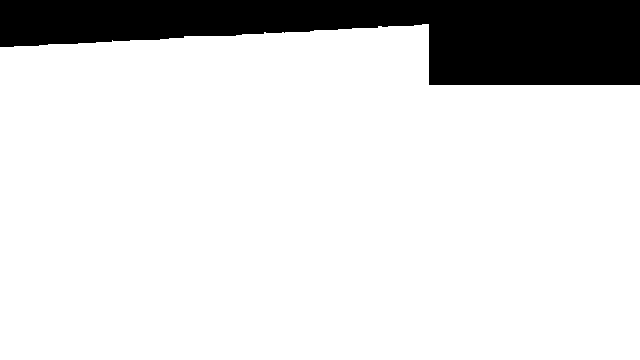
\includegraphics[width=0.4\textwidth]{frameCancha.png}
\end{figure}

\begin{figure}[!ht]
  \caption{M\'ascara de la cancha en el frame 90}
  \centering
    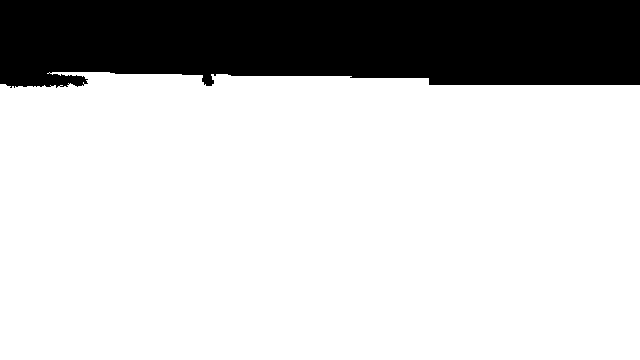
\includegraphics[width=0.4\textwidth]{frameCancha90.png}
\end{figure}

\begin{figure}[!ht]
  \caption{M\'ascara de la varianza en el frame 1}
  \centering
    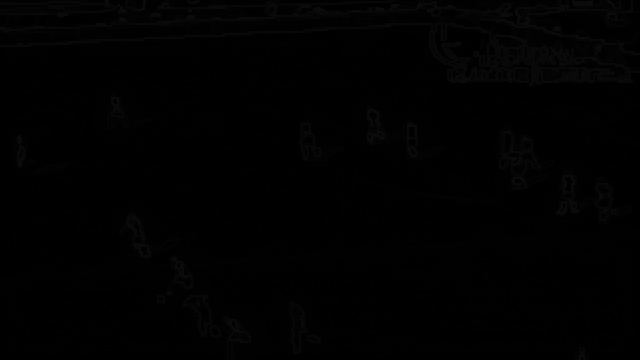
\includegraphics[width=0.4\textwidth]{frameVarianza.png}
\end{figure}

\begin{figure}[!ht]
  \caption{M\'ascara de la varianza en el frame 90}
  \centering
    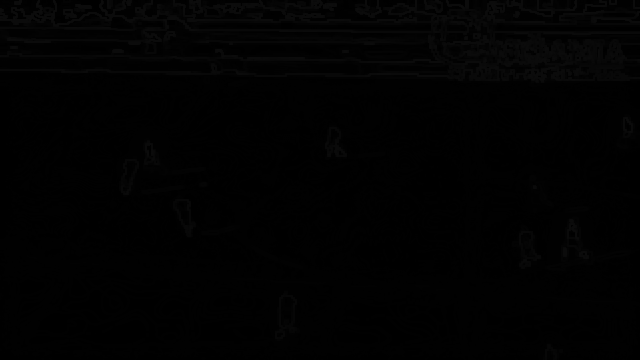
\includegraphics[width=0.4\textwidth]{frameVarianza90.png}
\end{figure}

\begin{figure}[!ht]
  \caption{Resultado final en el frame 1}
  \centering
    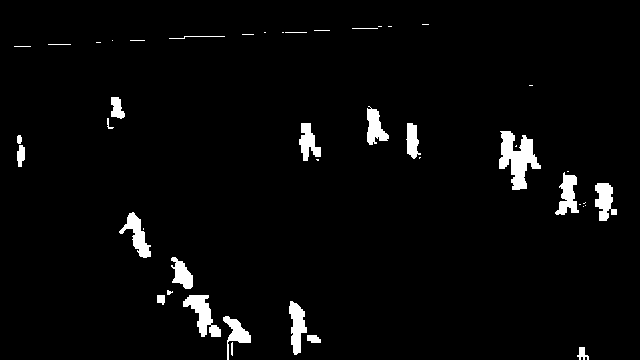
\includegraphics[width=0.4\textwidth]{frameFinal.png}
\end{figure}

\begin{figure}[!ht]
  \caption{Resultado final en el frame 90}
  \centering
    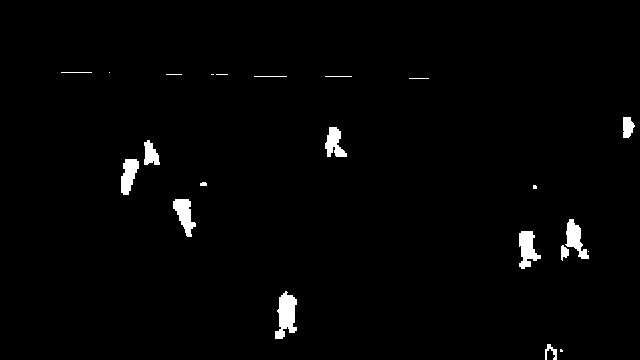
\includegraphics[width=0.4\textwidth]{frameFinal90.png}
\end{figure}

\newpage

\section{Conclusiones}

\begin{itemize}
\item La forma en la que esta dise\~nado el lenguaje \emph{Octave} lo hace muy pr\'actico para el manejo de se\~nales.
\item Dado que las matrices son un tipo de dato nativo del lenguaje, se facilita mucho el manejo y manipulaci\'on de imagenes, ya que estas se convierten en matrices num\'ericas.
\item Otro aspecto que se facilita por las matrices como tipo de dato primitivo, es la automatizaci\'on de recorridos de estructuras de datos. Dado que las matrices son tipos de datos primitivos, se elimina la necesidad de ciclos y/o ciclos anidados \emph{(fors dentro de fors o whiles)} para recorrer las matrices.
\item El lenguaje presenta una manera muy pr\'actica y f\'acil de agregar las librer\'ias necesarias.
\end{itemize}

\section{Referencias}

\begin{thebibliography}{99}

\bibitem{Community} Community, T. O.-F. (2009, June 7). \emph{Documentation}. Retrieved August 17, 2016, from \texttt{http://octave.sourceforge.net/docs.html}
\bibitem{GNU Octave} W, J. (1996). \emph{GNU octave}. Retrieved August 17, 2016, from \texttt{https://www.gnu.org/software/octave/doc/v4.0.1/}
\bibitem{Octave} \emph{Octave - preface}. Retrieved August 17, 2016, from \texttt{http://www.math.utah.edu/docs/info/octave\_1.html\#SEC27}
\end{thebibliography}

\end{document}
